\documentclass[10pt,a4paper,sans]{moderncv}
\moderncvstyle{banking}
\moderncvcolor{black}
\nopagenumbers{}

\usepackage[utf8]{inputenc}
\usepackage[top=0.15cm, bottom=0cm, left=0.25cm, right=0.25cm]{geometry}
\usepackage{ragged2e}
\usepackage{multicol}
\usepackage{enumitem}
\usepackage{amssymb}
\usepackage{fontawesome5}
\usepackage{xcolor}
\usepackage{hyperref}
\hypersetup{colorlinks=true, urlcolor=blue}

% Custom cventry
\newcommand*{\customcventry}[7][.10em]{%
\begin{tabular}{@{}l}
    {\bfseries #4} \\
    {\itshape #3}
\end{tabular}
\hfill
\begin{tabular}{l@{}}
    {\bfseries #5} \\
    {\itshape #2}
\end{tabular}
\ifx&#7&%
\else{\\
\begin{minipage}{\maincolumnwidth}%
    \footnotesize#7%
\end{minipage}}\fi%
\par\addvspace{#1}
}

\begin{document}

% Ultra-compact header: photo left (not in margin), title/info centered and bigger
\hspace*{0.03\textwidth}% less horizontal space before photo (10% bump back)
\begin{minipage}[c]{0.13\textwidth}
  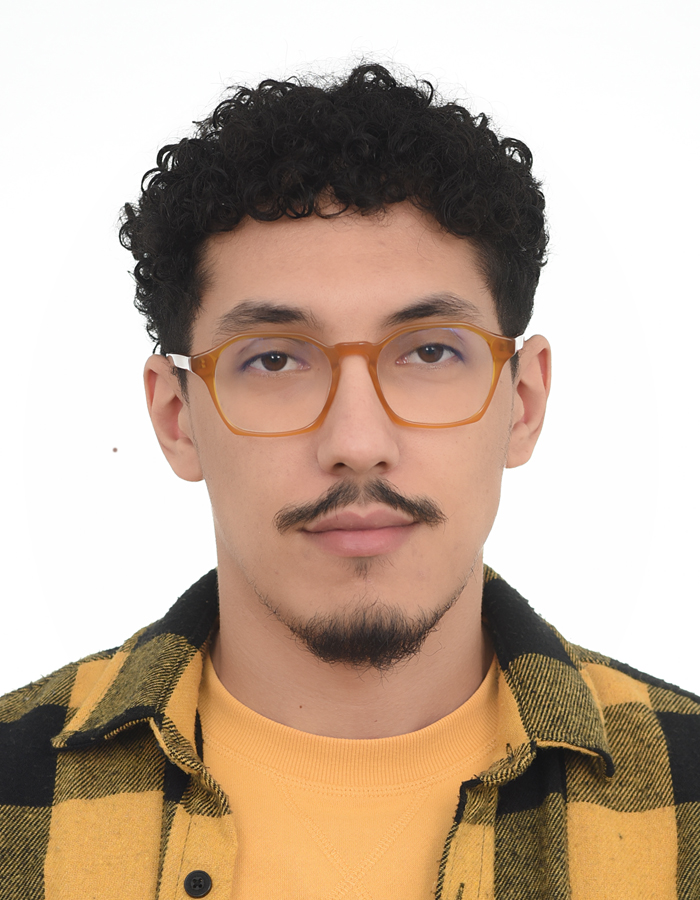
\includegraphics[width=0.85\linewidth]{images/ahmed.jpg}
\end{minipage}%
\hfill
\begin{minipage}[c]{0.84\textwidth}
  \begin{center}
    {\fontsize{20}{22}\selectfont\textbf{Ahmed MAKROUM}}\\[0.7em]
    {\fontsize{13.2}{15.4}\selectfont Développeur Full-Stack \& Ingénieur Logiciel} \\[0.5em] % <--- Ajouté ici
    {\fontsize{10.5}{12.3}\selectfont
      \faMobile\enspace +212 6 64 71 62 19 \quad
      \faEnvelope\enspace ahmedmakroum3@gmail.com \quad
      \faHome\enspace Casablanca, Maroc \\
      \faLinkedin\enspace \href{https://www.linkedin.com/in/ahmed-makroum/}{in/ahmed-makroum} \quad
      \faGithub\enspace \href{https://github.com/ahmedmakroum}{github.com/ahmedmakroum} \quad
      \faGlobe\enspace \href{https://makroum.website}{makroum.website}
    }\\[1em]
  \end{center}
\end{minipage}
\vspace{-16pt}

% PROFIL
\section{\fontsize{11}{12.1}\selectfont Profil}
\vspace{-7pt}
Ingénieur d’état en informatique et réseaux, je développe des applications web et mobiles complètes, côté client et serveur, en privilégiant la clarté, l’utilisabilité et la fiabilité, avec une expérience des outils cloud, de l’hébergement et du CI/CD. Je cherche un poste où je peux créer des outils concrets, utiles et accessibles.

% EXPÉRIENCE
\vspace{-17pt}
{\renewcommand{\labelitemi}{\raisebox{0.2ex}{\scalebox{1.15}{$\bullet$}}} % +15% size for bullets here only
\section{\fontsize{11}{12.1}\selectfont Expérience}
\vspace{-3pt}

\customcventry{03/2025 ‐ 08/2025}{\href{https://www.allianz.ma}{Allianz Maroc}}{Data Engineer}{}{}{
\begin{itemize}[leftmargin=0.8cm, itemsep=-2pt, topsep=0pt, partopsep=0pt, parsep=0pt]
\fontsize{10.5}{12.3}\selectfont
\item Développement et maintenance d’une application web de gestion des règlements de santé, utilisée quotidiennement par les équipes métier. Architecture microservices (Spring Boot, Next.js) avec authentification sécurisée (keycloack), gestion fine des rôles et interfaces responsives.
\item Conception et déploiement de pipelines de données (NiFi, Spark) pour automatiser l’extraction, le nettoyage et le chargement des données issues des systèmes d’assurance, remplaçant un processus manuel.
\item Intégration de sources de données hétérogènes dans un entrepôt PostgreSQL, consolidant plusieurs flux métiers, et création de dashboards interactifs avec Metabase pour visualiser les indicateurs clés et faciliter la prise de décision.
\end{itemize}}
  
\customcventry{06/2024 ‐ 08/2024}{\href{https://boti.education/}{BOTI School}}{Data Engineer}{}{}{
\begin{itemize}[leftmargin=0.8cm, itemsep=-2pt, topsep=0pt, partopsep=0pt, parsep=0pt]
\fontsize{10.5}{12.3}\selectfont
\item Développement d’un pipeline ETL distribué avec Apache Beam sur Google Cloud pour traiter des millions de logs utilisateurs.
\item Structuration de données issues de buckets GCP, rendant possible une analyse comportementale fiable.
\item Conception de dashboards automatisés via Looker, adoptés par l’équipe produit pour prioriser les évolutions.
\end{itemize}}

\customcventry{06/2023 ‐ 08/2023}{\href{https://6solutions.com/}{6solutions}}{Web and Mobile Developer}{}{}{
\begin{itemize}[leftmargin=0.8cm, itemsep=-2pt, topsep=0pt, partopsep=0pt, parsep=0pt]
\fontsize{10.5}{12.3}\selectfont
\item Développement d’une plateforme de consulting multi-services (juridique, médical, financier).
\item Front-end réalisé avec Angular, back-end avec Spring Boot.
\item Conception et déploiement de la version mobile de l’application en Flutter.
\end{itemize}}

\customcventry{07/2022 ‐ 08/2022}{\href{https://estatmar.ma/}{Finso}}{Game Developer}{}{}{%
\begin{itemize}[leftmargin=0.8cm, itemsep=-2pt, topsep=0pt, partopsep=0pt, parsep=0pt]
\fontsize{10.5}{12.3}\selectfont
\item Développement d’un jeu éducatif ludique, destiné aux enfants, pour introduire des notions simples de gestion et de stratégie.
\item Réalisation sous Unity avec un gameplay interactif, des animations soignées et une interface adaptée à un jeune public.
\end{itemize}}}
}

% PROJETS
\vspace{-12pt}
\section{\fontsize{11}{12.1}\selectfont Projets}
\vspace{-4pt}
\begin{itemize}[leftmargin=0.3cm, itemsep=-2pt, topsep=0pt, partopsep=0pt, parsep=0pt]
  \item \setlength{\parskip}{0pt}\textbf{JobTrack – Suivi de Candidatures} : Application web pour centraliser ses candidatures (CV, statuts, commentaires), avec recherche temps réel, tri dynamique et statistiques d’avancement. (Next.js, Tailwind, MongoDB, Cloudinary)
  
\item \textbf{Application de Suivi de Contrats d’Assurance} : Interface web permettant aux équipes métier de rechercher et suivre les contrats via une API connectée au système interne de l’entreprise, avec affichage structuré et filtres dynamiques. (React, Express.js)

  \item \setlength{\parskip}{0pt}\textbf{Outil Collecte de Feedback Interne} : Outil web avec interface Angular et backend Spring Boot pour soumettre, filtrer et exporter des feedbacks, avec gestion des rôles et stockage structuré. (Angular, Spring Boot, PostgreSQL)

  \item \setlength{\parskip}{0pt}\textbf{Prompt Engineering Extension} : Extension en JavaScript pour améliorer les prompts sur les sites d’IA (ChatGPT, Claude, Gemini…), en proposant des suggestions ciblées (clarté, contexte, précision). (JavaScript)

\end{itemize}


% FORMATION
\vspace{-18pt}
\section{\fontsize{11}{12.1}\selectfont Formation}
\vspace{-4pt}
\customcventry{2020 -- 2025}{\href{https://emsi.ma}{\textbf{EMSI – École Marocaine des Sciences de l’Ingénieur}}}{Diplôme d’Ingénieur en Informatique et Réseaux option MIAGE \\ (Méthodes Informatiques Appliquées à la Gestion des Entreprises)}{}{}{}
\customcventry{Juil. 2024 ‐ Sep. 2024}{\href{https://www.alxafrica.com}{\textbf{ALX Academy}}}{Diplôme de Formation en Intelligence Artificielle et Prompt Engineering}{}{}{ALX AiCE – AI Fundamentals}

% CERTIFICATIONS
\vspace{-16pt}
\section{\fontsize{11}{12.1}\selectfont Certifications}
\vspace{-5pt}
\textit{Certifications obtenues via Coursera.}
\begin{itemize}[leftmargin=0.3cm, itemsep=-2pt, topsep=0pt, partopsep=0pt, parsep=0pt]
    \item \textbf{\href{https://www.coursera.org/account/accomplishments/verify/G178XXP17WQA}{Machine Learning with Python}} (IBM)
    \item \textbf{\href{https://www.coursera.org/account/accomplishments/records/M5RKGX36BAVA}{IBM Data Engineering}} (IBM)
    \item \textbf{\href{https://google.com}{Building Scalable Java Microservices with Spring Boot and Spring Cloud}} (Google Cloud)
    \item \textbf{\href{https://www.coursera.org/account/accomplishments/verify/EK5SJM3YM7PX}{Introduction to Big Data with Spark and Hadoop}} (IBM)
    \item \textbf{\href{https://www.coursera.org/account/accomplishments/specialization/B4RCUAYCUG49}{Python for Everybody Specialization}} (University of Michigan)
    \item \textbf{\href{https://www.coursera.org/account/accomplishments/records/G867SJLRFQS2}{Google Business Intelligence}} (Google)
\end{itemize}

% COMPÉTENCES
\vspace{-16pt}
\section{\fontsize{11}{12.1}\selectfont Compétences}
\vspace{-6pt}
\begin{itemize}[leftmargin=0.3cm, itemsep=-2pt, topsep=0pt, partopsep=0pt, parsep=0pt]
    \item \textbf{Web/Mobile} : React, Next.js, Flutter, Spring boot, Apis REST
    \item \textbf{SGBD} : Conception et interrogation de bases SQL et NoSQL (PostgreSQL, MongoDB, Cassandra)
    \item \textbf{Programmation} : Python, SQL, Java, TypeScript, tests unitaires (Selenium, JUnit)
    \item \textbf{DevOps et Cloud} : Docker, Kubernetes, Git, CI/CD, Linux
    \item \textbf{Visualisation} : Metabase, Superset, Power BI
    \item \textbf{Soft Skills} : Travail d’équipe, communication, adaptabilité, résolution de problèmes
\end{itemize}

% LANGUES
\vspace{-16pt}
\section{\fontsize{11}{12.1}\selectfont Langues}
\vspace{-16pt}
\begin{multicols}{2}
\begin{itemize}[leftmargin=0.3cm, itemsep=-2pt, topsep=0pt, partopsep=0pt, parsep=0pt]
    \item Anglais – Courant
    \item Français – Courant
    \item Arabe – Maternelle
    \item Espagnol – Notions
\end{itemize}
\end{multicols}

% FOOTER

\vspace{-22pt}
\begin{center}
    {\fontsize{9}{11}\selectfont\color{gray}
   Pour plus d'informations sur mon travail, visitez mon~
    \faLinkedin~\href{https://www.linkedin.com/in/ahmed-makroum/}{LinkedIn}~ou~\faGithub~\href{https://github.com/ahmedmakroum}{GitHub}.}
\end{center}

\end{document}

